\documentclass{ximera}

%\usepackage{todonotes}

\newcommand{\todo}{}

\usepackage{esint} % for \oiint
\ifxake%%https://math.meta.stackexchange.com/questions/9973/how-do-you-render-a-closed-surface-double-integral
\renewcommand{\oiint}{{\large\bigcirc}\kern-1.56em\iint}
\fi


\graphicspath{
  {./}
  {ximeraTutorial/}
  {basicPhilosophy/}
  {functionsOfSeveralVariables/}
  {normalVectors/}
  {lagrangeMultipliers/}
  {vectorFields/}
  {greensTheorem/}
  {shapeOfThingsToCome/}
  {dotProducts/}
  {partialDerivativesAndTheGradientVector/}
  {../productAndQuotientRules/exercises/}
  {../normalVectors/exercisesParametricPlots/}
  {../continuityOfFunctionsOfSeveralVariables/exercises/}
  {../partialDerivativesAndTheGradientVector/exercises/}
  {../directionalDerivativeAndChainRule/exercises/}
  {../commonCoordinates/exercisesCylindricalCoordinates/}
  {../commonCoordinates/exercisesSphericalCoordinates/}
  {../greensTheorem/exercisesCurlAndLineIntegrals/}
  {../greensTheorem/exercisesDivergenceAndLineIntegrals/}
  {../shapeOfThingsToCome/exercisesDivergenceTheorem/}
  {../greensTheorem/}
  {../shapeOfThingsToCome/}
  {../separableDifferentialEquations/exercises/}
  {vectorFields/}
}

\newcommand{\mooculus}{\textsf{\textbf{MOOC}\textnormal{\textsf{ULUS}}}}

\usepackage{tkz-euclide}
\usepackage{tikz}
\usepackage{tikz-cd}
\usetikzlibrary{arrows}
\tikzset{>=stealth,commutative diagrams/.cd,
  arrow style=tikz,diagrams={>=stealth}} %% cool arrow head
\tikzset{shorten <>/.style={ shorten >=#1, shorten <=#1 } } %% allows shorter vectors

\usetikzlibrary{backgrounds} %% for boxes around graphs
\usetikzlibrary{shapes,positioning}  %% Clouds and stars
\usetikzlibrary{matrix} %% for matrix
\usepgfplotslibrary{polar} %% for polar plots
\usepgfplotslibrary{fillbetween} %% to shade area between curves in TikZ
%\usetkzobj{all}
\usepackage[makeroom]{cancel} %% for strike outs
%\usepackage{mathtools} %% for pretty underbrace % Breaks Ximera
%\usepackage{multicol}
\usepackage{pgffor} %% required for integral for loops



%% http://tex.stackexchange.com/questions/66490/drawing-a-tikz-arc-specifying-the-center
%% Draws beach ball
\tikzset{pics/carc/.style args={#1:#2:#3}{code={\draw[pic actions] (#1:#3) arc(#1:#2:#3);}}}



\usepackage{array}
\setlength{\extrarowheight}{+.1cm}
\newdimen\digitwidth
\settowidth\digitwidth{9}
\def\divrule#1#2{
\noalign{\moveright#1\digitwidth
\vbox{\hrule width#2\digitwidth}}}




% \newcommand{\RR}{\mathbb R}
% \newcommand{\R}{\mathbb R}
% \newcommand{\N}{\mathbb N}
% \newcommand{\Z}{\mathbb Z}

\newcommand{\sagemath}{\textsf{SageMath}}


%\renewcommand{\d}{\,d\!}
%\renewcommand{\d}{\mathop{}\!d}
%\newcommand{\dd}[2][]{\frac{\d #1}{\d #2}}
%\newcommand{\pp}[2][]{\frac{\partial #1}{\partial #2}}
% \renewcommand{\l}{\ell}
%\newcommand{\ddx}{\frac{d}{\d x}}

% \newcommand{\zeroOverZero}{\ensuremath{\boldsymbol{\tfrac{0}{0}}}}
%\newcommand{\inftyOverInfty}{\ensuremath{\boldsymbol{\tfrac{\infty}{\infty}}}}
%\newcommand{\zeroOverInfty}{\ensuremath{\boldsymbol{\tfrac{0}{\infty}}}}
%\newcommand{\zeroTimesInfty}{\ensuremath{\small\boldsymbol{0\cdot \infty}}}
%\newcommand{\inftyMinusInfty}{\ensuremath{\small\boldsymbol{\infty - \infty}}}
%\newcommand{\oneToInfty}{\ensuremath{\boldsymbol{1^\infty}}}
%\newcommand{\zeroToZero}{\ensuremath{\boldsymbol{0^0}}}
%\newcommand{\inftyToZero}{\ensuremath{\boldsymbol{\infty^0}}}



% \newcommand{\numOverZero}{\ensuremath{\boldsymbol{\tfrac{\#}{0}}}}
% \newcommand{\dfn}{\textbf}
% \newcommand{\unit}{\,\mathrm}
% \newcommand{\unit}{\mathop{}\!\mathrm}
% \newcommand{\eval}[1]{\bigg[ #1 \bigg]}
% \newcommand{\seq}[1]{\left( #1 \right)}
% \renewcommand{\epsilon}{\varepsilon}
% \renewcommand{\phi}{\varphi}


% \renewcommand{\iff}{\Leftrightarrow}

% \DeclareMathOperator{\arccot}{arccot}
% \DeclareMathOperator{\arcsec}{arcsec}
% \DeclareMathOperator{\arccsc}{arccsc}
% \DeclareMathOperator{\si}{Si}
% \DeclareMathOperator{\scal}{scal}
% \DeclareMathOperator{\sign}{sign}


%% \newcommand{\tightoverset}[2]{% for arrow vec
%%   \mathop{#2}\limits^{\vbox to -.5ex{\kern-0.75ex\hbox{$#1$}\vss}}}
% \newcommand{\arrowvec}[1]{{\overset{\rightharpoonup}{#1}}}
% \renewcommand{\vec}[1]{\arrowvec{\mathbf{#1}}}
% \renewcommand{\vec}[1]{{\overset{\boldsymbol{\rightharpoonup}}{\mathbf{#1}}}}

% \newcommand{\point}[1]{\left(#1\right)} %this allows \vector{ to be changed to \vector{ with a quick find and replace
% \newcommand{\pt}[1]{\mathbf{#1}} %this allows \vec{ to be changed to \vec{ with a quick find and replace
% \newcommand{\Lim}[2]{\lim_{\point{#1} \to \point{#2}}} %Bart, I changed this to point since I want to use it.  It runs through both of the exercise and exerciseE files in limits section, which is why it was in each document to start with.

% \DeclareMathOperator{\proj}{\mathbf{proj}}
% \newcommand{\veci}{{\boldsymbol{\hat{\imath}}}}
% \newcommand{\vecj}{{\boldsymbol{\hat{\jmath}}}}
% \newcommand{\veck}{{\boldsymbol{\hat{k}}}}
% \newcommand{\vecl}{\vec{\boldsymbol{\l}}}
% \newcommand{\uvec}[1]{\mathbf{\hat{#1}}}
% \newcommand{\utan}{\mathbf{\hat{t}}}
% \newcommand{\unormal}{\mathbf{\hat{n}}}
% \newcommand{\ubinormal}{\mathbf{\hat{b}}}

% \newcommand{\dotp}{\bullet}
% \newcommand{\cross}{\boldsymbol\times}
% \newcommand{\grad}{\boldsymbol\nabla}
% \newcommand{\divergence}{\grad\dotp}
% \newcommand{\curl}{\grad\cross}
%\DeclareMathOperator{\divergence}{divergence}
%\DeclareMathOperator{\curl}[1]{\grad\cross #1}
% \newcommand{\lto}{\mathop{\longrightarrow\,}\limits}

% \renewcommand{\bar}{\overline}

\colorlet{textColor}{black}
\colorlet{background}{white}
\colorlet{penColor}{blue!50!black} % Color of a curve in a plot
\colorlet{penColor2}{red!50!black}% Color of a curve in a plot
\colorlet{penColor3}{red!50!blue} % Color of a curve in a plot
\colorlet{penColor4}{green!50!black} % Color of a curve in a plot
\colorlet{penColor5}{orange!80!black} % Color of a curve in a plot
\colorlet{penColor6}{yellow!70!black} % Color of a curve in a plot
\colorlet{fill1}{penColor!20} % Color of fill in a plot
\colorlet{fill2}{penColor2!20} % Color of fill in a plot
\colorlet{fillp}{fill1} % Color of positive area
\colorlet{filln}{penColor2!20} % Color of negative area
\colorlet{fill3}{penColor3!20} % Fill
\colorlet{fill4}{penColor4!20} % Fill
\colorlet{fill5}{penColor5!20} % Fill
\colorlet{gridColor}{gray!50} % Color of grid in a plot

\newcommand{\surfaceColor}{violet}
\newcommand{\surfaceColorTwo}{redyellow}
\newcommand{\sliceColor}{greenyellow}




\pgfmathdeclarefunction{gauss}{2}{% gives gaussian
  \pgfmathparse{1/(#2*sqrt(2*pi))*exp(-((x-#1)^2)/(2*#2^2))}%
}


%%%%%%%%%%%%%
%% Vectors
%%%%%%%%%%%%%

%% Simple horiz vectors
\renewcommand{\vector}[1]{\left\langle #1\right\rangle}


%% %% Complex Horiz Vectors with angle brackets
%% \makeatletter
%% \renewcommand{\vector}[2][ , ]{\left\langle%
%%   \def\nextitem{\def\nextitem{#1}}%
%%   \@for \el:=#2\do{\nextitem\el}\right\rangle%
%% }
%% \makeatother

%% %% Vertical Vectors
%% \def\vector#1{\begin{bmatrix}\vecListA#1,,\end{bmatrix}}
%% \def\vecListA#1,{\if,#1,\else #1\cr \expandafter \vecListA \fi}

%%%%%%%%%%%%%
%% End of vectors
%%%%%%%%%%%%%

%\newcommand{\fullwidth}{}
%\newcommand{\normalwidth}{}



%% makes a snazzy t-chart for evaluating functions
%\newenvironment{tchart}{\rowcolors{2}{}{background!90!textColor}\array}{\endarray}

%%This is to help with formatting on future title pages.
\newenvironment{sectionOutcomes}{}{}



%% Flowchart stuff
%\tikzstyle{startstop} = [rectangle, rounded corners, minimum width=3cm, minimum height=1cm,text centered, draw=black]
%\tikzstyle{question} = [rectangle, minimum width=3cm, minimum height=1cm, text centered, draw=black]
%\tikzstyle{decision} = [trapezium, trapezium left angle=70, trapezium right angle=110, minimum width=3cm, minimum height=1cm, text centered, draw=black]
%\tikzstyle{question} = [rectangle, rounded corners, minimum width=3cm, minimum height=1cm,text centered, draw=black]
%\tikzstyle{process} = [rectangle, minimum width=3cm, minimum height=1cm, text centered, draw=black]
%\tikzstyle{decision} = [trapezium, trapezium left angle=70, trapezium right angle=110, minimum width=3cm, minimum height=1cm, text centered, draw=black]


\title{Inverse Functions}

\begin{document}

\begin{abstract}
one-to-one
\end{abstract}
\maketitle





Just like numbers, functions have an arithmetic.  They have all of the usual number operations, plus one more.  Functions also have \textbf{\textcolor{purple!85!blue}{composition}} as an operation.

Just like number operations have identity numbers, $0$ and $1$, composition has an identity function - the identity function: $Id(x) = x$.




Around these identity elements, we define inverses.






\begin{itemize}
\item The additive inverse of $a$ is the number that when added to $a$ results in $0$.  Our symbol is $-a$, which we call the \textbf{\textcolor{blue!55!black}{opposite}} of $a$.
\item The multiplicative inverse of $a$ is the number that when multiplied to $a$ results in $1$.  Our symbol is $\frac{1}{a}$ or $a^{-1}$, which we call the \textbf{\textcolor{blue!55!black}{reciprocal}} of $a$.
\item The composition inverse of a function $f$ is the function that when composed with $f$ gives the identity function. Our symbol is $f^{-1}$, which we call the \textbf{\textcolor{blue!55!black}{inverse}} of $f$.
\end{itemize}





\begin{definition} \textbf{\textcolor{green!50!black}{The Inverse of a Function}} 


Let $f$ be a one-to-one function with domain $D$, range $R$, and pairs $(d, f(d))$.

Then the inverse function of $f$ is a function with domain $R$, range $D$, and pairs $(f(d), d)$.


The inverse of $f$ is denote as $f^{-1}$.

\end{definition}






\textbf{Notation Warning:} We reuse and overuse notation in Mathematics.  This is an example.  Sometimes $f^{-1}$ means reciprocal and sometimes $f^{-1}$ means inverse function.  The correct interpretation depends on the context in which it used.













\section*{Inverse Functions}




Composition glues function pairs together producing a third function.

Let $In$ and $Out$ be two functions and $Out \circ In$ their composition.


Pairs in $In$ look like $(a, In(a))$.   The composition then interprets $In(a)$ as a member of the domain of $Out$.  $Out$ connects $In(a)$ to $Out(In(a))$.   The composition, $Out \circ In$ just ignores the middle part.  The composition sees $a$ as a domain number and then $Out(In(a))$ as the range partner.


Suppose we are in a situation where $Out(In(a)) = a$, which means the composition is the identity function.  That would tell us that $Out$ is the inverse function of $In$.  $Out = In^{-1}$.

Then we would have pairs inside $In$ looking like $(a, In(a))$ and pairs inside $In^{-1}$ looking like $(In(a), a)$.  The inverse function just reverses the order pair. \\


\textbf{\textcolor{blue!75!black}{$\blacktriangleright$}}  The inverse function is just the reverse of the original function. \\


This brings up an important issue.


\begin{warning} \textbf{\textcolor{red!70!black}{Inverse Functions}} 

Reversing the pairs of a function does not always produce a function.


\end{warning}




\begin{example} Squaring Function


The squaring function has the formula $Sq(a) =a^2$ with \textbf{$\mathbb{R}$} as its domain.

It contains the two pairs: $(2, 4)$ and $(-2, 4)$.



If we reverse these pairs, then the inverse function would contain the pairs: $(4, 2)$ and $(4,-2)$.

This would violate the function rule.  We would have a domain number in two pairs.

\end{example}



Just like with numbers, some functions don't have inverses.  Like, $0$ just doesn't have a multiplicative inverse.






\section*{One-to-One}


Some functions just don't have an inverse, because they have a range number in two pairs.  This is fine for the function, but when reversing the pairs to obtain the inverse funciton, then that range number turns into a domain number in two pairs.


For a function to have an inverse, every range number must be in only one pair.



\begin{definition} \textbf{\textcolor{green!50!black}{One-to-One}}    


A function is said to be \textbf{one-to-one} if each range number is in exactly one pair.


\end{definition}



Or, an equivalent definition:

\begin{definition} \textbf{\textcolor{green!50!black}{One-to-One}}   


A function, $f$, is said to be \textbf{one-to-one} if 


\[    f(a) = f(b) \rightarrow a = b           \]


\end{definition}





This definition says that if two function values are equal, then they couldn't have come from two different domain numbers.  They came from the same domain number. So, each function value is in exactly one pair.








\begin{example} Linear Functions

If $C$ is a constant function, then it is not one-to-one and thus doesn't have an inverse. \\


If $C$ is a nonconstant linear function, then it has a formula like $C(x) = a \cdot x + b$ where $a \ne 0$.


Then $C^{-1}(t) = \frac{1}{a} \cdot t - \frac{b}{a}$


\begin{explanation}



The composition is 

\[  (C \circ C^{-1})(w) = C(C^{-1})(w) =     a \cdot \left(\frac{1}{a} \cdot w - \frac{b}{a}\right) + b  = w \]


and the other way


\[  (C^{-1} \circ C)(y) = C^{-1}(C(y)) =     \frac{1}{a} \cdot (a \cdot y + b) - \frac{b}{a}  = y \]


\end{explanation}


\end{example}








\begin{example} Square



The squaring function has the formula $Sq(k) = k^2$ with \textbf{$\mathbb{R}$} as its domain. It doesn't have an inverse.




\begin{image}
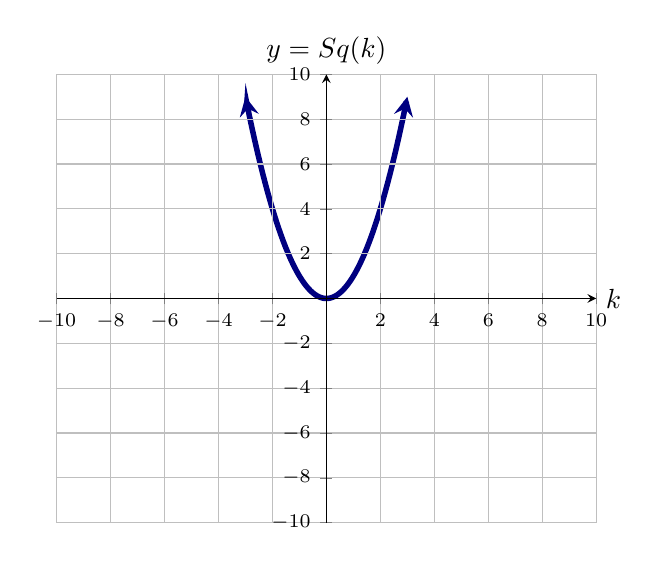
\begin{tikzpicture}
  \begin{axis}[
            domain=-10:10, ymax=10, xmax=10, ymin=-10, xmin=-10,
            axis lines =center, xlabel=$k$, ylabel={$y=Sq(k)$}, grid = major,
            ytick={-10,-8,-6,-4,-2,2,4,6,8,10},
            xtick={-10,-8,-6,-4,-2,2,4,6,8,10},
            yticklabels={$-10$,$-8$,$-6$,$-4$,$-2$,$2$,$4$,$6$,$8$,$10$}, 
            xticklabels={$-10$,$-8$,$-6$,$-4$,$-2$,$2$,$4$,$6$,$8$,$10$},
            ticklabel style={font=\scriptsize},
            every axis y label/.style={at=(current axis.above origin),anchor=south},
            every axis x label/.style={at=(current axis.right of origin),anchor=west},
            axis on top
          ]
          

            \addplot [line width=2, penColor, smooth,samples=100,domain=(-3:3),<->] {x^2};

         

  \end{axis}
\end{tikzpicture}
\end{image}


The graph contains the two points: $(2, 4)$ and $(-2, 4)$.  

They are at the same vertical height, which means they represent the same function value.


The two points lie on the same horizontal line.








\begin{image}
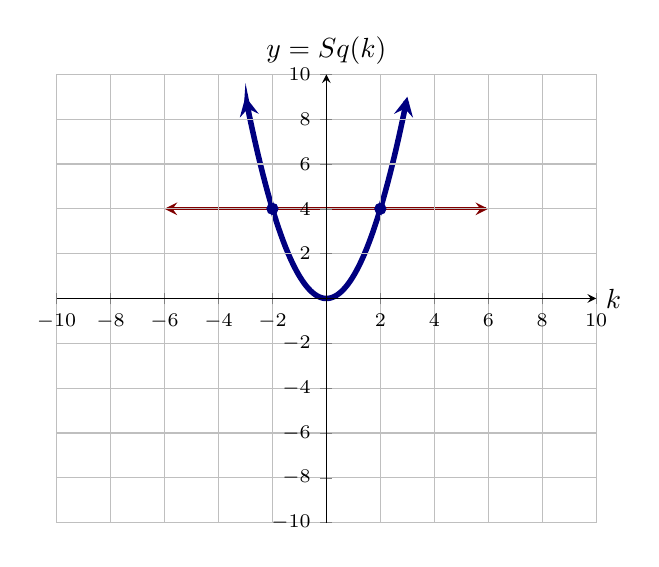
\begin{tikzpicture}
  \begin{axis}[
            domain=-10:10, ymax=10, xmax=10, ymin=-10, xmin=-10,
            axis lines =center, xlabel=$k$, ylabel={$y=Sq(k)$}, grid = major,
            ytick={-10,-8,-6,-4,-2,2,4,6,8,10},
            xtick={-10,-8,-6,-4,-2,2,4,6,8,10},
            yticklabels={$-10$,$-8$,$-6$,$-4$,$-2$,$2$,$4$,$6$,$8$,$10$}, 
            xticklabels={$-10$,$-8$,$-6$,$-4$,$-2$,$2$,$4$,$6$,$8$,$10$},
            ticklabel style={font=\scriptsize},
            every axis y label/.style={at=(current axis.above origin),anchor=south},
            every axis x label/.style={at=(current axis.right of origin),anchor=west},
            axis on top
          ]
          

            \addplot [line width=2, penColor, smooth,samples=100,domain=(-3:3),<->] {x^2};

            \addplot[color=penColor,fill=penColor,only marks,mark=*] coordinates{(2,4)};
            \addplot[color=penColor,fill=penColor,only marks,mark=*] coordinates{(-2,4)};
            \addplot [line width=1, penColor2, smooth,samples=100,domain=(-6:6),<->] {4};

         

  \end{axis}
\end{tikzpicture}
\end{image}






\end{example}




\begin{definition} \textbf{\textcolor{green!50!black}{Horizontal Line Test}}  


A function's graph passes the horizontal line test if there are no horizontal lines that intersect the graph more than once.


A function is one-to-one if its graph passes the horizontal line test.

\end{definition}
















\section*{Salvaging}


Functions that are not one-to-one do not have an inverse.

We can't fix this situation, but we can salvage pieces. \\







\begin{example} Squaring Function


The squaring function has the formula $Sq(k) = k^2$ with \textbf{$\mathbb{R}$} as its domain. It doesn't have an inverse.

However, we can get a partial inverse, by restricting the domain.

The implied domain of $Sq(k) = k^2$ is \textbf{$\mathbb{R}$}.  We will restrict this to just the nonnegative numbers: $[0, \infty)$.






\begin{image}
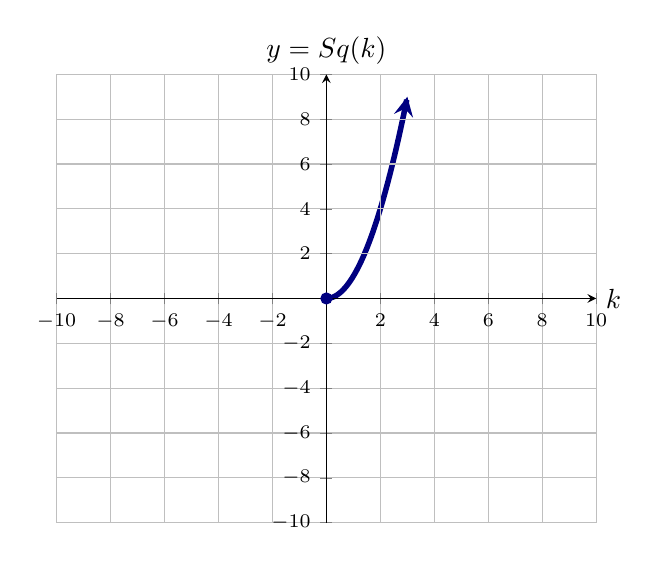
\begin{tikzpicture}
  \begin{axis}[
            domain=-10:10, ymax=10, xmax=10, ymin=-10, xmin=-10,
            axis lines =center, xlabel=$k$, ylabel={$y=Sq(k)$}, grid = major,
            ytick={-10,-8,-6,-4,-2,2,4,6,8,10},
            xtick={-10,-8,-6,-4,-2,2,4,6,8,10},
            yticklabels={$-10$,$-8$,$-6$,$-4$,$-2$,$2$,$4$,$6$,$8$,$10$}, 
            xticklabels={$-10$,$-8$,$-6$,$-4$,$-2$,$2$,$4$,$6$,$8$,$10$},
            ticklabel style={font=\scriptsize},
            every axis y label/.style={at=(current axis.above origin),anchor=south},
            every axis x label/.style={at=(current axis.right of origin),anchor=west},
            axis on top
          ]
          

            \addplot [line width=2, penColor, smooth,samples=100,domain=(0:3),->] {x^2};
            \addplot[color=penColor,fill=penColor,only marks,mark=*] coordinates{(0,0)};

         

  \end{axis}
\end{tikzpicture}
\end{image}



Now, it has the square root function as an inverse.




\begin{image}
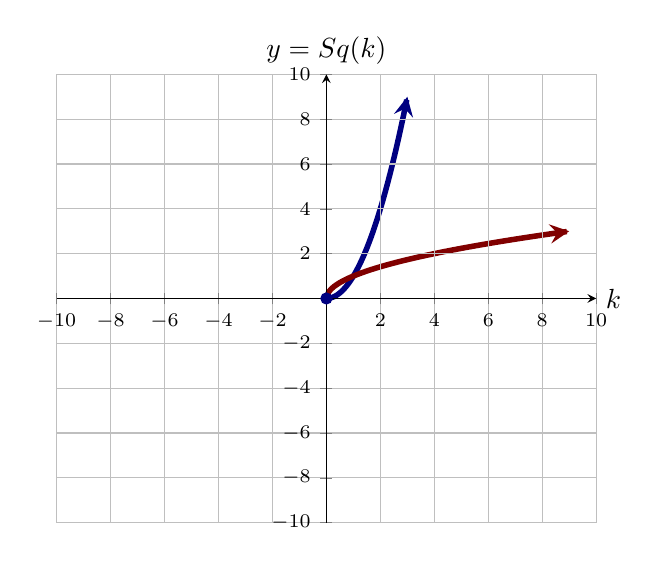
\begin{tikzpicture}
  \begin{axis}[
            domain=-10:10, ymax=10, xmax=10, ymin=-10, xmin=-10,
            axis lines =center, xlabel=$k$, ylabel={$y=Sq(k)$}, grid = major,
            ytick={-10,-8,-6,-4,-2,2,4,6,8,10},
            xtick={-10,-8,-6,-4,-2,2,4,6,8,10},
            yticklabels={$-10$,$-8$,$-6$,$-4$,$-2$,$2$,$4$,$6$,$8$,$10$}, 
            xticklabels={$-10$,$-8$,$-6$,$-4$,$-2$,$2$,$4$,$6$,$8$,$10$},
            ticklabel style={font=\scriptsize},
            every axis y label/.style={at=(current axis.above origin),anchor=south},
            every axis x label/.style={at=(current axis.right of origin),anchor=west},
            axis on top
          ]
          

            \addplot [line width=2, penColor, smooth,samples=100,domain=(0:3),->] {x^2};
            \addplot[color=penColor,fill=penColor,only marks,mark=*] coordinates{(0,0)};

            \addplot [line width=2, penColor2, smooth,samples=100,domain=(0:9),->] {sqrt(x)};



         

  \end{axis}
\end{tikzpicture}
\end{image}




Since the inverse function has the reverse pairs of the original function, its graph is a reflection across the graph of the identity function: $y = Id(k) = k$.






\begin{image}
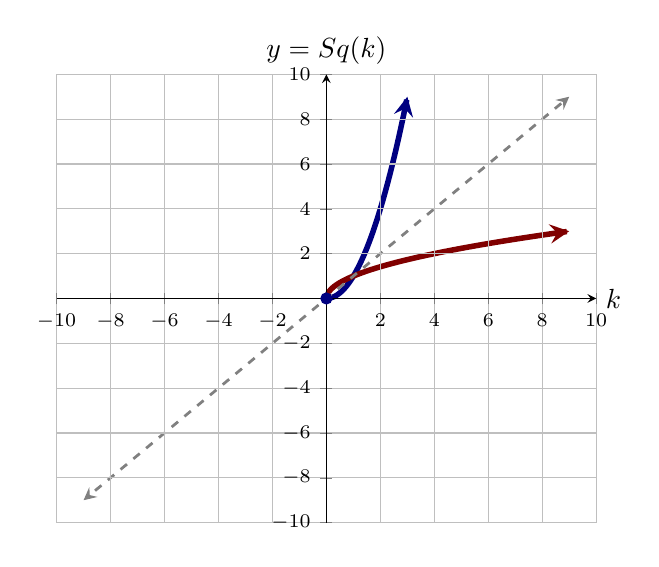
\begin{tikzpicture}
  \begin{axis}[
            domain=-10:10, ymax=10, xmax=10, ymin=-10, xmin=-10,
            axis lines =center, xlabel=$k$, ylabel={$y=Sq(k)$}, grid = major,
            ytick={-10,-8,-6,-4,-2,2,4,6,8,10},
            xtick={-10,-8,-6,-4,-2,2,4,6,8,10},
            yticklabels={$-10$,$-8$,$-6$,$-4$,$-2$,$2$,$4$,$6$,$8$,$10$}, 
            xticklabels={$-10$,$-8$,$-6$,$-4$,$-2$,$2$,$4$,$6$,$8$,$10$},
            ticklabel style={font=\scriptsize},
            every axis y label/.style={at=(current axis.above origin),anchor=south},
            every axis x label/.style={at=(current axis.right of origin),anchor=west},
            axis on top
          ]
          

            \addplot [line width=2, penColor, smooth,samples=100,domain=(0:3),->] {x^2};
            \addplot[color=penColor,fill=penColor,only marks,mark=*] coordinates{(0,0)};

            \addplot [line width=2, penColor2, smooth,samples=100,domain=(0:9),->] {sqrt(x)};
            \addplot [line width=1, gray, dashed,samples=200,domain=(-9:9),<->] ({x},{x});



         

  \end{axis}
\end{tikzpicture}
\end{image}





\end{example}


















\begin{example} Inverse Function


Let $H(t) = 3t - 5$. \\

Then $H^{-1}(x)$ is a function such that $H \circ H^{-1} = Id$ \\


We are looking for a function, $H^{-1}$, such that $(H \circ H^{-1})(k) = H(H^{-1}(k)) = 3 H^{-1}(k) - 5 = k$ \\



$H$ is linear and $Id$ is linear, therefore $H^{-1}$ should be linear.

Let's start building.  $H^{-1}(x)$ should look like $a \cdot x + b$.  The leading coefficient of $H^{-1}$, $a$, should be $\frac{1}{3}$.


$H^{-1}(x) =\frac{1}{3} x + b$


That would gets us $H(H^{-1}(k)) = 3 (\frac{1}{3}x + b) - 5 = x + 3b - 5 $


We need $3b - 5 = 0$ or $b = \answer{\frac{5}{3}}$.


$H^{-1}(x) =\frac{1}{3} x + \frac{5}{3}$



\end{example}




\begin{question} Inverse


Suppose $T$ is a one-to-one function with $T(4) = 5$. Then which inverse value do we know?


\begin{multipleChoice}
\choice {$T^{-1}(-4) = -5$}
\choice {$T^{-1}\left(\frac{1}{4}\right) = \frac{1}{5}$}
\choice {$T^{-1}(-5) = -4$}
\choice[correct] {$T^{-1}(5) = 4$}
\end{multipleChoice}

\end{question}






















\begin{center}
\textbf{\textcolor{green!50!black}{ooooo-=-=-=-ooOoo-=-=-=-ooooo}} \\

more examples can be found by following this link\\ \link[More Examples of Function Algebra]{https://ximera.osu.edu/csccmathematics/precalculus1/precalculus1/functionAlgebra/examples/exampleList}

\end{center}






\end{document}
